Il seguente codice plotta la funzione \\
\lstinputlisting{cap_1/es13/es13.m}
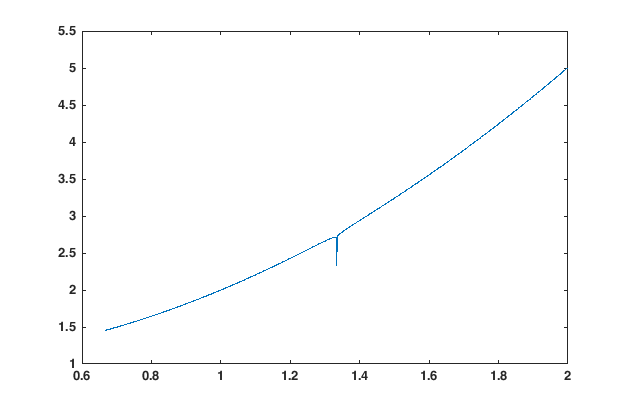
\includegraphics[scale=0.8]{cap_1/es13/es13.png}\\
Il  motivo per cui f(x) in x=4/3 è pari ad un valore finito risiede nel fatto che 4/3 è un numero razionale periodico.
Il calcolatore memorizzerà fl(4/3) con un approssimazione determinata dalla precisione macchina in uso.
Calcolando infatti l'espressione mostrata a riga 12 del listato abbiamo questo output:\\   2.220446049250313e-16\\
Questo valore, analiticamente dovrebbe essere 0 ma, dato che la memorizzazione di 4/3 non è precisa, il valore della funzione nel punto verrà finito.
